\chapter{Antecedents of Modern Urban Rent Theory: Rent and Production} \label{chapter-rent}

\epigraph{Of the concrete forms of income that have usually been classed as surplus, the rent of land was the earliest to be defined; and so prominent a position has been given to it that the terms `rent' and `surplus' have come to be used interchangeably.}{Alvin Saunders Johnson, 1902 \cite{johnsonRentModernEconomic1902}}
\epigraph{The law of rent has become an obstacle to scientific progress: it has retarded the attainment of a true theory of distribution ... % Yet it is itself capable of affording such a theory. 
The principle that has been made to govern the income derived from land actually governs those derived from capital and from labor. 
}{John Bates Clark, 1891 \cite{clarkDistributionDeterminedLaw1891}}

% WHAT BELONGS IN INTRO? RICARDO AND HIS HISTORICAL CONTEXT SEEMS TO GO INTO MORE DEPTH. NEED TO FOCUS OF INTRODUCING RENT, ITS DEFINITION AND IT'S RELATIONSHIP TO LOCATIONAL VALUE AND DISTRIBUTION OF SURPLUS AND GENERALLY RELATIONSHIP. 
% FINANCIALIZATION OF HOUSING MARKET IS IN SPACE - LOCATIONAL...

% STREAM OF BENEFITS... DRAWING OUT THE RELATIONSHIP BETWEEN DIFFERENT TYPES OF VALUE OF LAND AND HOW LOCATIONAL VALUE MATTERS ... IS IN RICARDO AS EXTENSIVE MARGIN - 
% 2 MEANINGS OF MARGIN WHICH RELATE TO THE TWO FORMS OF VALUE PROVIDED BY LAND.


% To build a model of financialization, we need to bring in a concept of rent, that was central in classical economics, but has not been as important in formal neoclassical modeling.
% which is described in the next chapter and to which this thesis contributes. 
% We trace the development of theories of income distribution through the classical and neoclassical periods to provide context to our contribution to the development of a modern urban rent theory.  
% We correct that omission because they are
% Along the way, we also explain how the competing approach to distribution, has perhaps unintentionally left most

In an urban economy, land provides benefits in the form of housing, and places for work, storage, commerce and recreation. Location matters in an urban economy because value is generated by bringing people and activities together. The value of a piece of land in a city derives, not from the richness of the soil, but from the richness of the activities is supports and because of the people and activities it provides access to.   

The value of land is accounted for by the economic concept of rent. \Gls{rent}, in economic theory is not the amount a tenant pays a landlord every month, nor is it simply a payment for using land or another facility. %For economists, the word normally means the \gls{surplus} income produced by a scarce factor of production that is created by nature. 
%NEW \Gls{rent}, in economic theory is therefore, not the amount a tenant pays a landlord every month. It  nor is it simply a payment for access to the services provided by the land or another facility.  The economist's notion thus overlaps with, but is not identical with common usage. 
For modern economists, the word extends to include the \gls{surplus} income produced by any scarce factor of production that is created by nature that has locational value. People pay a high price for housing near the center of a city because there is limited %nature did not make much
land close to the city center and being close to urban jobs and amenities is valuable. The extra cost to be close to the center is an \gls{economic rent}. %It was not created by the landlord, but it appears as income for the landlord. Thus 
Natural resources like mineral deposits generate rents just as productive land does.  %In a similar way, people pay a higher price for housing near  urban jobs and amenities. Land near the centre of a city provides locational services that are far more valuable than any of its potential agricultural services. Because nature did not make much land close to the city center, these locational services are scarce and command a high price. The extra cost to be close to the center is an \gls{economic rent}. 
The natural talents of a sports star also generate rents. % In general, the locational element is ignored but, IT IS ALWAYS OR GENERALLY AT PLAY?. Even in the sports example. 
It may seem odd to think of a football player like Lionel Messi as having a locational value, but if his services cannot be delivered to a market willing to pay to watch football, his services as a footballer have little or no value. Economists talk about scarce talents using the concept of rent, developed to understand land rents.  

In the thesis we use the concept of rent to model how financialization captures a share of urban productivity. %surplus value. Financialization is about capturing the surplus in an urban economy. 
The concept of rent provides us with a theory for understanding the distribution of surplus.  If financialization of the urban housing market is directed to capturing the stream of economic surpluses generated by the city, % urban agglomeration, 
the theory of rent provides a basis for understanding the allocation of surpluses.


In this chapter, we build a bridge from \gls{classical rent theory} to the modern theory of urban rent, which this thesis works to develop. To do this, %we trace the development of antecedents to the work on modern urban rent theory developed in this thesis, beginning with classical tradition of rent, and tracing through the development of the neoclassical tradition, and modern theories of production. 
% and how. This leads directly to 
we discuss classical and neoclassical theories of rent and production. 



% The land itself is not better but the location is. %It was not created by the landlord, but it appears as income for the landlord. Thus 



%

%Property and land have multifaceted benefits that include both what you are using it for and the value of what it is in proximity to.


% for those with financial assets.
% Financialization is the capture of surplus. Rent is key to how economists have studied the distribution of the surplus. % It was central in classical economics.
% In order to model what's happening in financialization, we need the concept of rent. https://www.overleaf.com/project/606a6b286ae1c9f203fadab5
% In 1902 Alvin Saunders Johnson \cite{johnsonRentModernEconomic1902} summarized the relationship between rent and surplus in the economic literature as follows: 
% \begin{quotation}Of the concrete forms of income that have usually been classed as surplus, the rent of land was the earliest to be defined; and so prominent a position has been given to it that the terms ''rent'' and ''surplus'' have come to be used interchangeaby.\end{quotation} 

 



% In this thesis, we identify what are essentially \glspl{classical rent} in the urban system and examine their distribution to develop a model of financialization of the urban housing market. 
% We bring in the concept of rent because it is necessary background for our examination of the impact of \gls{financialization} on urban productivity. 
% ***E OR MAYBE OPEN WITH THIS? OR: Economics is the study of ___. It is concerned with production (i.e. ___ and distribution (ie. ___) 
% We use the \gls{Cobb-Douglas} function %, which is used to cross this entire range of literature to illustrate each link and to show how our model is directly connected with this broad collection of linked theories. 
% The \gls{Cobb-Douglas} function is a production function, expressing the output produced, in terms of inputs such as labour and capital.
% Our model connects to the results in this chapter at four points:

% In the following chapters we will discuss the three pieces of theory needed to build a model of financialization, rent, urban spatial models, and growth theories. From there, we will bring these things together into a formal model in Part~\ref{part-model}.
 

\section{Classical theories of rent and the distribution of surplus value}

% The question of how wealth is created and distributed has been central to Economics since the discipline emerged. %** ^E ADD GENERAL STATEMENT ABOUT THIS OR MAYBE CUT THIS SENTENCE
Prior to the industrial revolution, most people in Europe lived on and worked the land, primarily producing food, with ownership concentrated in the hands of a few landowners. In this context, land provides a stream of benefits in the form of agricultural products and therefore landownership formed the basis of wealth, political power, and social distinction.  % the land-owning class in the era of the classical economists. % Property ownership has been a central form of wealth throughout history. % one of central forms of  wealth and means of building wealth 
% As the primary source of food, power comes from food, which was the main product. 
%  ADD EXPLANATION % Land ownership traditionally defined the ruling classes. The king would give land as reward. Land is what you would fight wars for. The agricultural surplus , the surplus from the land what allowed civilization and cities to form. Before the industrial revolution, the surplus of  agricultural land. taking ownership used to consolidate wealth and power, in feudalism ownership of land set apart ruling classes/aristocracy, . As pearl buck said "land is everything.." or quote that "the only way to create intergenerational wealth is the rare company that or property ownership.  GIVE EXPLANATION HISTORY OR SUMMARY
% More recently the expansion of European economies across the globe brought huge amounts of land into play and combined with rapidly falling transportation costs, led to a society, especially in the labour-scarce settler societies of North America and Australia with  widely distributed property and  home ownership. 

For early economists, % of the early stage of the industrial revolution, % it seemed clear that 
all wealth came from the land. The Physiocrats in particular, a school of economists in 18th-century France, emphasized that land is the source of all wealth, that only agricultural labour was productive.\footnote{They argued, based on the productivity of land, that government policy should not interfere with the operation of natural economic laws. Within this framework, they were the first to frame labour as the source of value. Marx, extending the approach to the industrial economy, generalized the analysis, treating industrial labour as generating a surplus as well, as we discuss in \ref{section-rent-and-industrial-capital}.} Tradespeople, professionals, clergy, and aristocrats were nonproductive. Landowners controlled access to the means of production and charged for access. 

Rent theory originated in this land-based agricultural society. The income landowners extracted was what economists called \gls{economic rent}, or \gls{land rent}. Early economic analysis focused on land and on the rents to understand the allocation of the surplus product of the land. Rent was the value of the productivity of the land itself after costs. Since costs included the costs of transporting produce to market, land rent was always based on the location of the land. % IS THIS TRUE??? EDIT::
Given the importance of land to overall economic productivity, the theory of rent emerged as a primary way of understanding distribution of wealth in this period. 

It was described early as political economy.
%, and economic analysis naturally focused on the distribution of the rent. % surpluses of the land, rent.
% The physiocratic school of economics was the first to see labour as the sole source of value but, for the physiocrats, in the context of the prevalent European rural society of the time, only agricultural labour created a surplus. 

\subsection{Historical development of classical rent theory}

% FOOTNOTE? Classical rent theory originated with thinkers such as Richard Cantillon (1680s--1734), Fran\c{c}ois Quesnay (1694--1774), the marquis de Mirabeau (1715--1789), Anne-Robert-Jacques Turgot (1727--1781) and Adam Smith (1723--1790), and received its classic statement in Ricardo (1772--1823). Nearly contemporaneous thinker, Johann Heinrich von Th\"unen (1783--1850) developed a planning model to guide the location of economic activities for an urban-agricultural society. A version of that model was reinvented in urban geography by William Alonzo.

David Ricardo provided the canonical presentation of the classical theory of rent \cite{ricardoEssayInfluenceLow1815} in 1815. 
 Ricardo defines rent in relation to who claims the surplus productivity of the land, %this idea about the productivity of land, and who claims that value, 
saying ``[b]y rent I always mean the remuneration given to the landlord for the use of the original power of the land'' \cite{ricardoEssayInfluenceLow1815}. The key term in that definition is ``the original power of the land.'' In the classical tradition, rent is the surplus produced by labour using land that is claimed by landowners by virtue of their ownership of the land. The price of the corn would include payment for working the land and for transporting, storing, and selling the product, but the part that was rent would be a payment for the virtue of the land not of the landlord.

For Ricardo, %and for the classical economics in general, 
\gls{land rent} is thus a kind of \gls{surplus value}, that is an amount available after the costs of production have been paid, the term rent came to be used interchangeably with this more general concept in much of the classical work on rent and the term rent has been used in a more general sense to other kinds of surplus value, as well as land rents. % Surplus value is essentially profit, the value beyond the costs.
Alvin Saunders Johnson, wrote in 1902, ``[o]f the concrete forms of income that have usually been classed as surplus, the rent of land was the earliest to be defined; and so prominent a position has been given to it that the terms `rent' and `surplus' have come to be used interchangeably'' \cite{johnsonRentModernEconomic1902}. 
The economist's notion thus overlaps with, but is not identical with common usage. 

In Ricardo's time, economic rent and the rent paid by farmers to use the land were almost interchangeable. Landowners `rented out' land. The level of rent charged might not be exactly the economic rent, but in a labour-surplus economy\footnote{Between 1604 and 1914 over 5,200 enclosure Bills were enacted by Parliament which related to just over a fifth of the total area of England, amounting to some 6.8 million acres. From the 1750s enclosure by parliamentary Act became the norm. In Scotland  between 1750 to 1860 the  Highland Clearances  evicted a significant number of tenants in the Scottish Highlands and Islands, mostly in two phases from 1750 to 1860. Enclosures and clearances created a large pool of essentially minimum wage labour that supported industrialization and drove British migrations to the colonies.} landlords had enormous bargaining power, and charged tenant farmers rents that tended to approximate the value of the \gls{surplus}. %, and rent as a price tended to approximate \gls{economic rent}. 
 

Ricardo used this concept of rent to build out a theory designed to answer the social question `who gets the surplus?' This was an approach to understanding the distribution of wealth.% and explaining inequality.%the inequality the economists were seeing.
 \footnote{For Ricardo this theory provided insight into whether Britain should open its doors to corn from the colonies. This was the debate over the Corn Laws (1794-1846), a set duties on grain imports into Britain to protect British agriculture from outside competition. In Britain, ``corn'' was the generic name for cereal crops. The full title of Ricardo's essay explains his purpose" \textit{An Essay on the Influence of a Low Price of Corn on the Profits of Stock, Showing the Inexpediency of Restrictions on Importation: With Remarks on Mr Malthus' Two Last Publications: `An Inquiry into the Nature and Progress of Rent,' and `The Grounds of an Opinion on the Policy of restricting the Importation of Foreign Corn.'''}} His model explained the distribution of the product of the earth among the ``three classes of the community'' which is to say, to the owners of land, labour, and capital.
\footnote{
Ricardo was interested, in particular, in the division of the surplus among the classes of society:  
% \begin{quotation}   
 ``The produce of the earth---all that is derived from its surface by the united application of labour, machinery, and capital, is divided among three classes of the community; namely, the proprietor of the land, the owner of the stock or capital necessary for its cultivation, and the labourers by whose industry it is cultivated. ...  But in different stages of society, the proportions of the whole produce of the earth which will be allotted to each of these classes, under the names of rent, profit, and wages, will be essentially different''  \cite{ricardoEssayInfluenceLow1815}. CHECK SOURCE.
% \end{quotation}
}
He worked in a time of rising poverty and inequality.\footnote{The economic transformations of the period increased overall wealth, although in many cases the living condition of the working class declined.} in the context of the primarily agricultural economic system during increasing globalization of trade and the early stages of the industrial revolution in Northern Europe.\footnote{The Industrial Revolution is usually described as beginning around 1760 and having significantly transformed society by about 1820--1840.} % In this period, the study of \gls{political economy} was emerging as a subject of study that focused on understanding trade, wealth, and government.\footnote{CHECK/REPHRASE? Prior to this, international relationships centred on studies of the military. As colonization changed the relationship between countries and trade became central, the study of \gls{political economy} became more significant.}

 





% It's easy enough to see how this concept would evolve into the two different usages of the term rent. Because it is the profit for the land, which is related to payments for the land. At the time, the feudal ownership structures meant that the value of the land was structured differently. Tenants did not pay to occupy the land the way that people and businesses do today. Rather the value of owning land was reflected in the distribution from production. The term later split to reflect both the way land is currently valued (i.e rent payments to occupy) and the surplus value that was how land was valued in the period of clssical econmics with it's feadul structures. Rent became payment to landlord because under feudalism, the surplus went to the landlords. Thenn the term diverged into the two distinct meanings used colloquially and in a technical context by Economists ) 

%The profit now accrues to the landowner, and we call it land rent. For Ricardo, it was obvious that the land-owning class captured the land rent.

\subsection{Locational value in agricultural markets}
% who picks up vegetables at the farm gate, transports them into town, and sells them to a storekeeper. He pays the farmer at one end of the trip and is paid at the other. 

The central role of locational value in the theory of \gls{rent} can be illustrated with the story of a carter, who purchases agricultural products, for instance potatoes, from farms, and carries them, on a cart, to sell in town. 
% (Carter's expensive dirrectly change the value of the land, dependant on proximity, because they change expenses.
The carters expenses depend on how close they are to---reflect the expense incured depending ot proximity to market. 
% Imagine an  town in Ricardo's context, surrounded by potato farms, with people who pulled carts to carry potatoes to sell at a market. 
% Imagine there is one person who owns the only cart in the region that can be used to move potatoes. Now imagine that this monopoly carter notices that 
There is a price for potatoes in town and a lower price at the farm gate, so the carter can buy potatoes from farmers, transport them to town, and resell them at a higher price in the urban market. What remains of the price gap, after subtracting labour and vehicle costs, is profit.  

\begin{figure}[htb]
\begin{center}
     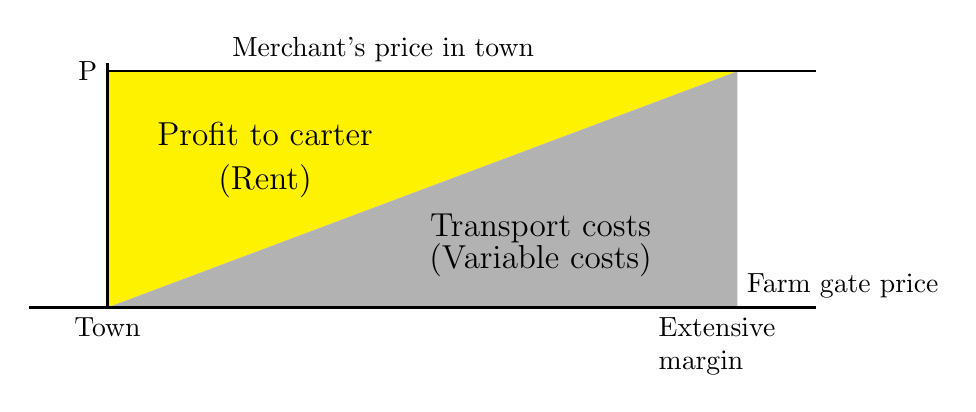
\begin{tikzpicture}[domain=0:2]
%\draw[thick,color=gray,step=.5cm, dashed] (-0.5,-.5) grid (3,3);
%\draw[line width=.01, green ] (0,0) -- (10,0) node[right  ] {Distance};
\node at (1,0) [below] {Town};
\fill[yellow]  (1,0) --(9,3)--(1,3) --cycle;
\fill[gray!60] (9,3) --(1,0)--(9,0) --cycle;

\draw[thick ] (1,3)node[left]{P}  -- (10,3);\node at (4.5,3)[above ] {Merchant's price in town} ;
\draw[thick ] (0,0)  -- (10,0); 

%\draw[thick,color=red] (1.5,0) -- (1.5,1) node[below right] {Fixed cost} -- (1.5,1.5) --(10,3.25)node[above left] {total cost};
\draw[thick] (1,0) -- (1,3.1) ;
\node[below,text width=2cm]at (9,0) {Extensive margin};
%\draw[ultra thick, blue,<-> ] (3,1.8) -- (3,2.5)node[left] {annual rent at a} -- (3,3) ; 
\node at (9,0)[above right] {Farm gate price};
\node  at (6.5,1){\large Transport costs};
\node  at (6.5,.6){\large (Variable costs)};
\node  at (3.,2.2){\large Profit to carter};
\node  at (3.,1.6){\large (Rent)};
\end{tikzpicture} 
\caption[Ricardo's theory of extensive margin.]{Ricardo's theory of the extensive margin using transportation costs to emphasize the similarity between rent in classical theory and in the Alonzo model, developed in the next chapter, Chapter~\ref{chapter-space}. Transport costs, the lighter, yellow area, take a share of the profit for vegetables sold in the town}
\label{fig-rent-ricardo}
\end{center}
\end{figure}

The land rent declines with distance from the town. Beyond certain distance, the costs of the trip will eat up all profit. That is the farthest distance the carter will go to purchase potatoes. That distance is Ricardo's \gls{extensive margin}.\footnote{Ricardo carefully distinguished the \gls{intensive margin} and the \gls{extensive margin}. The extensive margin is where the most distant land worth cultivating given the cost of transportation. The intensive margin, on the other hand, can be seen as the limit to increasing the productivity of a particular piece of land by applying fertilizer, draining, or paying more workers. It's the improvements possible to increase productivity of the land.} % The extensive margin provides a key insight  into modern urban tent theory. 
% ELABORATE ON WHY EXTENSIVE MARGIN MATTERS. - QQQ FERTILITY VS DISTANCE TO MARKET
FLIP DESCRIPTION AND CHECK ALIGNS WITH OTHER FIGURES. Figure~\ref{fig-rent-ricardo}, shows the total transportation costs as the lighter, yellow area. The area below the yellow triangle is profit for the carter. The carter makes a `profit' on the trip to the farm nearest to town, a lower profit farther from town, and no profit on any farms beyond this point.\footnote{Note the similarity with Alonzo's urban model, illustrated in Figure~\ref{fig-rent-alonzo}, in Chapter~\ref{chapter-space}.} 

Together these two triangles represent the net farm-gate value of the `product of the earth,' but only the lower triangle is \gls{surplus}. It was termed the `produit net' by the Physiocrats. In modern supply and demand analysis it would be recognized as `producer surplus,' the difference between what a producer gets for a good and what they would be willing to accept. This surplus is what can be allocated to the landlord, the carter, the merchant or the consumer. 

% The surplus declines for distance, it also declines for less fertile land. %, where there is a higher cost of production. 
Just as there is more surplus for land closer to market, there is more surplus for land that is more productive. In most of the discussion, Ricardo emphasized differential land fertility rather than distance to market. % Only some land produces a surplus of income. 
Good land produced more market value for the same cost as the poorest land in production. The poorest land in production just barely justified the cost of production, by definition. If it cost more to grow than not, there would be no incentive to cultivate the land. On the least productive land, after paying for labour and any other costs of production, there is no surplus left for the land owner. More fertile land generated more than the annual costs faced by a landowner. % RICARDO, PHISIOCRATS OR SOMEONE ELSE NOTED THIS?
The difference in earnings between the poorest land in production and a more fertile or better located field was what could be claimed as a surplus or rent. % the quantity that economists called rent. 

At the farthest point, whether in fertility or distance, what Ricardo called the extensive margin, land rent falls to zero. % It is barely worth cultivating the land. %Even fertile 
Farmers won't cultivate land beyond the extensive margin, because there is not profit. % the product cannot make % be transported to market at a profit. % Transportation costs and the price of produce in town determine the size of the  rent triangle, and the amount of rent captured by the land-owning class. %\footnote{The debate about the ``Corn Laws'' that Ricardo was engaged in was about whether Britain would allow wheat from Canada and Australia to enter, reducing the price of wheat and therefore reducing the income and influence of the land-owning class.} 
If the merchant's price goes up, or costs go down, the \gls{extensive margin} would move farther out, and more land would come into production.\footnote{This example illustrates the principle with % assumes that the land is 
uniformly productive and a single product. Johann Heinrich von Th\"unen, in \textit{The Isolated State} (\textit{Der isolierte Staat}), 1826, \cite{vonthunenIsolirteStaatBeziehung1826}), provided a more complex analysis based on the same principles.} % ***E ADD?? This graph is simplified to illustrate the concept.
% For simplicity, assume all farmers have the same cost of production, and the carters pay the farmer the farm gate price at the farm and receive the merchant price in town. 





\subsection{Rent and industrial capital} \label{section-rent-and-industrial-capital}
As the economy shifted  moved from overwhelmingly agricultural into the industrialization of the 18$^{th}$  and 19$^{th}$ century, it became increasingly important to theorize industrial production. A theory of value in which only land produced value was increasingly insufficient. 
 % It was central to the dominant mode of analysis and continued into early theorizing of industrialization.
% MARX IS LINK TO INDUSTRIAL CAPITALISM
% EARLY THEORIES OF INDUSTRIAL CAPITALISM ACTUALLY STILL CENTERED RENT, IT WAS THE NATURAL WAY TO UNDERSTAND THIS. SEE MARX, HENRY GEORGE EXTENSION TO THE CITY.
% There was a shift to industrial capitalism from an agricultural economy.
% There were some efforts to integrate rent in the analysis this new economic reality, like that by Marx. 
%Ricardo, agreeing with Malthus, essentially assumes that the wage is  just sufficient to reproduce the labouring class.\footnote{``In the natural advance of society, the wages of labour will have a tendency to fall, as far as they are regulated by supply and demand; for the supply of labourers will continue to increase at the same rate, while the demand for them will increase at a slower rate.''} He then explains the distribution of the fruits of labour on the land among the main classes of the economy.
%***E ADD CONTEXT like:
Early theories of rent and industrial production still centered rent in the classical sense. 

Karl Marx's work is an example of an analysis that generalized the classical approach to rent to the study of industrial capitalism, centered on industrial production. % of a system level of effects of shifts in structures of financial capital and financial instruments in an industrial economy. 
% , in a sense of a different iteration of financialization of the previously non-financial-but financialization embedded in production. % Later stories decoupled from production, with the financial structures coming to run on a logic of their own.
Marx, (1818--1883), was born three years after Ricardo published his \textit{Essay on the Price of Corn}. By the time Marx wrote % was displaying  his developing interest in economics  
at the radical newspaper, \textit{Rhineland News}, Ricardo had been dead 20 years, the industrial revolution had been underway for almost a century, and European economies were largely structured around manufacturing. 

 % ***E MORE ACCURATE TO SAY HE was exploring this because it was what he saw than shifted attention.
 In the manufacturing economy, the owners contribute the machinery, buildings, and even working capital to fund the workers until the product can be sold. % ***E FLESH OUT THIS DESCRIPTION OF THE KEY FEATURES OF TEH MANUFACTURING ECONMY. ALOS SPECIFCAL DEFINE CAPITAL CAN WHY IT MATTERS
 %This contribution must be accumulated from their profits in the preceding cycle of production,  and has to be reinvested once the revenues of the current round have come in and the bills have been paid. Marx actually describes a circuit of capital from its form as money to its form as physical capital. 
In Marx's analysis there's surplus labour, capital is scarce, and the scarce factor is owned by a special class, as in Ricardo's analysis---now the capitalists---who are able to appropriate the surplus value. %Like Ricardo,  Marx saw the appropriation of surplus as without moral justification. 

Marx pointed to an additional dynamic feature of capitalist systems---that productive capital is not fixed as land is, but  expands as surplus is reinvested. This creates an economy that can, and according to Marx must, grow. It also introduces challenges created by the capitalists' need to reinvest their growing accumulation of surplus value.\footnote{In some analysis, financialization of housing is part of an effort to find places to invest capitalist surplus value, for instance in David Harvey's work on the second circuit of capitalism \cite{GET_david_harvey}.} % It was not until 1867 that  the first volume of \textit{Das Kapital},  was published, pulling together 20 years of Marx's analysis of the capitalist economy. \textit{Das Kapital} proposes an explanation of the ``laws of motion'' of the mode of production from its origins to its future by describing the dynamics of the accumulation of capital. With topics such as the growth of wage labour, the transformation of the workplace, capital accumulation, competition, the banking system, the tendency of the rate of profit to fall, and land-rents.% ***E EXPLAIN WHAT THIS MEANS AND WHY IT MATTERS TO DISTRIBUTION. HOW IS IT DIIFFERENT OR SIMLAR TO WHAT WAS HAPPENING UNDER FEUDALISM? 
%He famously suggested that the expansion will eventually outrun the expansion of demand and the rate of return will fall, leaving capitalists unwilling to invest. % and creating a crisis. 

% ***E FILL OUT CRISIS % WHEN i GET TO HENRY GEORGE AND YOU MAKE THE DISTINCTION BETWEEN HIS VIEW OF WHAT WOULD CAUSE CRISIS AND MARX'S, i AM CONFUSED BECAUSE YOU DON'T FULLY ARTICULATE THE PROBLEM. I THINK THIS IS SOMETHING MISSING HERE, BUT YOU COULD ALSO CHANGE THE LINE IN THE GEORGE SECTION IF THIS IS NOT AS IMPORTANT. TO ADD YOU WOULD JUST NEED TO EXPLAIN HOW THE NEED FOR GROWTH ULTIMATELY CREATES A PROBLEM OR CRISIS. WHY IS DOES IT POSE CHALLENGES. 
%***E I ALSO THINGK THAT THIS LIST OF TOPICS IN THE BOOK IS A BIT OF AN ABRUPT END TO EXPLAINING MARX'S CONTRIBUTIONS. IT WOULD BE HELPFUL TO PAINT MORE OF A PICTURE OF WHAT HE DOES WITH THESE TOPICS. INCLUDING THE CRISIS THING BUT ALSO A BIT MORE GENERALLY. THE TRANSITION TO HOW YOU POSITION MARX IS CURRENTLY A BIT ABRUPT. 

% ADD? We see Marx as firmly part of the Classical tradition and a contributor to distributional theory.  Our work, linking urban rents to the dynamics of financial capital has one foot firmly  in the Ricardian and Marxian  tradition. Like Marx and Ricardo we explore how a particular type of surplus is distributed, how that might change, and the effect on society  ***E OF THE VARIOUS SYSTEMS OF DISTRIBUTION?. Like Marx and Ricardo we find that a functional approach to social classes provides a useful framework. Where Marx focused on industrial \gls{capital}, however, we focus on capital in a different form: \gls{financial capital}% ***E SEEMS TO BE A LOT MISSING HERE?

% ***E i FEEL LIKE IT WOULD BE USEFUL TO DESCRIBE THE CLASS BREAKDOWN IN MARX AS IT RELATES TO HOW THE DIFFERENT ROLES FIT INTO PRODUCTION. aLSO. WHAT HAPPENED TO THE IDEA OF LAND RENT IN THIS PERIOD AND IN MARX'S WORK SPECIFICALLY? dID HE IGNORE IT? EVEN IF HE DIDN'T USE THE CONCEPT, EXPLAIN HOW IT WOULD RELATE OR FIT (OR NOT FIT) INTO THIS CONCEPT)

\subsection{Rent and the city} 
With industrialization, economic activity increasingly grew around urban industrialized areas and factories, %. Land was no longer the central locus of growing economic output, 
and cities became increasingly important to economic analysis. Early understanding of the cities rising importance also centered the distributional insights of classical rent theory. % Rent was also central in the early economic understanding of this process of urbanization. 
% As Marx linked rent and industrial production, 
Henry George's work, in particular, linked rent to an understanding of urban surplus. % productivity. % /urban wealth/cuties. %and cities. 
% In economics Henry George's work links rents and space
% , but it has not been taken up to the degree that it could be. 
% ***E THIS SECTION FEELS A LITTLE SPARSE ON ECONOMIC ANALYSIS %YOU EXPLAIN GEORGE'S CONCLUSIONS CLEARLY, BUT I FEEL THIS WOULD BE STREGTHEN A LITTLE MORE CLARITY ABOUT HOW HE RE-INTRODUCE LAND RENT. WHAT WAS THE ANALYSIS / iNSIGHT EXACTLY? THEN GO INTO THE CONCLUSIONS HE DREW ABOUT WHAT SHOULD HAPPEN...

In 1879, Henry George (1839--1897), an influential American political economist, published his most famous work, \textit{Progress and Poverty} \cite{georgeProgressPovertyInquiry1973}. It sold millions of copies worldwide. George returned to land rent with a new insight based on the emergence of the capitalist city: the owners of urban land extract surplus in exactly the same way that owners of agricultural land do in Ricardo's analysis. ``[w]ith the growth of population, land grows in value, and the men who work it must pay more for the privilege.''  Where Marx saw the extravagant productivity of capital as the source of capitalist rent, George saw the extraction of wealth by land speculators as the mechanism that let owners claim surplus value. % would bring on crises.
  % ***E WHAT DID HE MEAN BY CRISIS? HOW DID HE COME TO BE CONCERNED ABOUT THIS? ALSO SINCE YOU ARE COMPARING WITH MARX's PREDICTIONS ABOUT CRISIS YOU NEED TO EXPLAIN MORE ABOUT MARX'S IDEAS OF CRISIS ABOVE
  % ***E Somewhere in HERE YOU MAY WANTED TO EXPLAIN SOCIALISM VS MARXISM... GEORGE IS SOCIALIST? MARX?? PUTTING IN THE CONTEXT OF HOW THOSE TRADITIONS WERE EMERGING MIGHT BE HELPFUL... I HAD THIS NOTE ON THE PAPER DRAFT... COULDN'T FIGURE OUT WHY SINCE YOU DON'T SAY GEORGE IS A SOCIALIST. bUT YOU DO LATER WHEN YOU EXPLAIN THE SHIFTS IN jb CLARK'S THINKING. IF YOU WANT TO CONTEXTUALIZE CLARK IN TERMS OF SOCIALISM ... BEST TO MAKE SURE YOU'VE EXPLAINED THAT GEORGE IS A SOCIALIST, WHAT THAT MEANS, AND THEN, SINCE MARX IS FAMOUSLY BUT CONFUSINGLY INTERCONNECTED WITH SOCIALISM YOU SHOULD EXPLAIN HOW HIS THINK AND (SEPARATELY) THE MOVEMENT NAMED AFTER HIM FIT IN) 
  % # ADD George also presented solutions to ____ 

George's work represents an important development in the theory of rent, for this work. The classical economists agreed that rents are unearned income. They did not emphasize, as George did, that land rents arise from labour's proximity to urban population and production.\footnote{To be fair, it was not lack of understanding, that the classical omission of urban rents reveals, but rather lack of interest in urban production, in a primarily agricultural context.} % in explicitly examining urban land rent from residential or even industrial purposes.} % George's work added a link to cities and distribution that this work takes up.  % Ricardo von Thunen, Marx, Cantillon all grasped the notion of proximity to the market as part of the source land rent. The discussions seem to not gone farther than discussions of diffeerential and rents, however.  I just am not aware of them explicitly examining urban land rent for residential or even industrial purposes. 

George's analysis has been taken up by major economic thinkers, and the core analysis has been widely accepted by economists across the discipline, and according to its proponents, it has important policy implications. Since land rent is not created by its owners, George argued that land rent should be seen as a social income---that it could be used to pay for the needs of the community.\footnote{George's emphasis on land rents parallels the view of the Physiocrats, who concluded that agricultural \gls{ground rents} should be the source of most or all taxes. They defined ground rent as that portion of all rent which is attributable only to the size and location of the parcel.} % The clearest statement of this view is found in \textit{Progress and Poverty} when he wrote ``We must make land common property.''
George's analysis led to the \gls{single tax} movement, which sought to shift all taxation to land  and resource rents.%Stiglitz formalized the conditions under which this should be taken up.  
\footnote{In 1977, Joseph Stiglitz identified the conditions in which Henry George's \gls{single tax} is  the only tax necessary to finance public expenditures, using Alonzo's relatively new urban model \cite{GET-stliglits_henry-georege-1979}.  %\footnote{Arnott, Richard J.; Joseph E. Stiglitz (November 1979). ``Aggregate Land Rents, Expenditure on Public Goods, and Optimal City Size'' (PDF). Quarterly Journal of Economics. 93 (4): 471--500. doi:10.2307/1884466. JSTOR 1884466. S2CID 53374401 }   
The logic is fairly simple: if the public good increases productivity or the attractiveness of a city, attracting more people or businesses, land rents rise, and investment in the public good should proceed until the marginal cost of the public good is equal to the increase in land rent it brings. The result is now called the \gls{Henry George theorem}.} %***E RELATE THIS TO YOUR THESIS. %I FEEL A BIT LOST IN WHAT YOU ARE SETTING UP HERE. COULD YO EXPLAIN HOW THEIS IS RELEVANT TO MODERN URBAN RENT THEORY? 
% ***E MAYBE MOVE UP THIS FOLLOWING PARAGRAPH? %THIS FEELS LIKE IT WOULD FIT WITH MORE DETAILED DESCRIPTION OF HIS ANALYSIS THAT I THINK SHOULD COME BEFORE HIS IDEAS ABOUT THE TAX. 
% The need to be near a market or prodduction center is easily seen by considering a population at the carrying capacity of the land with individuals supporting themselves using purely local resources. There can be no land rent in this case. If a city rises that must be supplied from those still on the land, land close enough to the city will generate land rent. The value of the land is created by proximity to the city.

%  no separate and comprehensive data are provided on the amounts of land rents and subsoil rents charged and earned, because they are not officially regarded as part of value-added, and consequently are not included in the calculation of GDP (except for the value of productive lease contracts)     https://en.wikipedia.org/wiki/Differential_and_absolute_ground_rent#Rent_in_macro-economics    \href{https://en.wikipedia.org/wiki/Differential_and_absolute_ground_rent#Rent_in_macro-economics}{Wikipediat article on differential rent}

\subsection{Rent in modern economic theory}
In modern economic theory, this classical concept of rent, has come through in a number of ways: 
% The concept of rent has remained central in economic analysis. For instance here are a few examples: 
% The classical idea of rent and rent has persisted and passed into modern economics in a number of forms. Several examples include: % ***E 
% MOVE DOWN suppressed as a concept as though it appears in a huge number of contexts, thought not under the name, but it appears not in the clasical
% drop land out of neoclaclasical analysis since were not focuse on fixed/unchangible factors
 % ADD BACK *** Modern economists generally focus  on the exchange price and the marginal conditions satisfied in exchange, which neoclassical economics explains more satisfactorily They appear to have abandoned rents as a central concept, but it  persists in slightly covert forms at the centre  neoclassical economics. 
\begin{enumerate}

    \item As we discuss in the introduction, first year students learn that the high salaries of sports stars are rents on their scarce talents. 

    \item The First Fundamental Theorem of Welfare Economics, proven independently by Kenneth Arrow \cite{arrowExtensionBasicTheorems1951}and  Gerald Debreu \cite{debreuCoefficientResourceUtilization1951}  in 1951, possibly the most significant theorem in the social sciences, demonstrates that perfectly competitive markets would maximize producer and consumer surplus, quantities that really are variants of rents.

    \item The theory of \gls{rent-seeking}  became the subject of durable interest among economists and political scientists after the publication of two influential papers on the topic by Gordon Tullock in 1967 \cite{tullockWelfareCostsTariffs1967}, and Anne Krueger \cite{kruegerPoliticalEconomyRentSeeking1974} in 1974. Rent-seeking occurs when an someone seeks to increase their own wealth without creating any benefits or wealth to the society. Financialization, as we use the term, is a variety of rent-seeking
    
    \item And, as we discuss in detail in Chapter~\ref{chapter-space}, the classical concept of rent is also at the heart of modern urban theory, although that work does not bring forward the distributional aspects of the classical analysis. The \gls{bid-rent curve}, the value of the bid, or what people will pay to live near the center, became a dominant device  in urban theory with William Alonzo's 1961 thesis \cite{alonzoTheoryUrbanLand1960} and the work that followed. %, although the idea has deep roots and others were exploring the principle at the same time.  % DEFINE BID RENT, LINK WITH REST OF THESIS.
\end{enumerate}
% SHORT CLASSICAL EXAMPLE. Or, in a modern example, professional sports players' income, above the opportunity cost they could get working at another position, is rent they capture for their skill.

These actually form the link with neoclassical analysis. We may want to put them later.

\begin{enumerate}
    \item Alfred Marshall identified industrial profits as a form of rents, terming them `quasi-rents' to emphasize that, unlike land rents, industrial profits would be expected to disappear over time as new firms entered the industry.
    
    \item First year students also learn about `consumer surplus' and `producer surplus' in supply and demand analysis. Both of these concepts are variants of rent and are essential in demonstrating the efficiency of a markets and the social losses due to \gls{monopoly}, \gls{monopsony}, regulation, and taxes. Consumer surplus is the sum of rents that accrue to the class of consumers (buyers). It is an \gls{inframarginal} quantity, like land  rent, that accrues to the class of landowners. It arises because consumers have differing capacity to produce  utility with the good, just as landowners have lands with different abilities to produce agricultural output. Producer surplus corresponds precisely to land rent in Figure~\ref{fig-rent-ricardo}.  
\end{enumerate}

\section{Neoclassical distribution theory}
% Rent now however competes with what is essentially another approach to distribution, developed through the neoclassical tradition. % This new approach is exciting and successful but in some ways displaces what went before. (our work is a synthesis)
% 
  % # NEED SOME MORE CONTEXT HERE. maybe atart by setting up the PERIOD WE ARE NOW MOVING INTO AND WHAT HAS SHIFTED IN THE ECONOMIC STRUCTURE? 

 
Despite the successes of rent as a way of explaining the distribution of the surplus. % industrial of rent.
Rent theory was eventually eclipsed by an approach that focused on the markets for the inputs used in industrial production. % Rent was displaced in the analysis of distribution, %It was eventually displaced in the neoclassical work of thinkers like John Bates Clark.
Classical theories of distribution showed that ownership of a scarce and non-produced factor, land, was the  basis of rent extraction by the class of landowners. Increasingly something else was happening in the industrial economy, that this older approach to distribution and rents did not seem to explain. 

\subsection{Distribution of the surplus of industrial production}
The neoclassical approach %Reason is that it
solved a core puzzle that was increasingly important to understanding the industrial economy and production. As industrial production became more important,  economists shifted their focus from who got the rents to how prices and especially the prices of factors of production were determined, and how the prices allocated to the factors of production related to surplus value.  
% WHAT IT IS 

Profits were a bit puzzling for the classical economist because their connection to land rents was not clear. Were profits just a part of land productivity captured by industrial producers as the earliest classical theorists argued, or were they  additional social surplus as the later classical theorists thought? Who claimed these surpluses and how did they develop over time? % ***E i DON'T UNDERSTAND WHY PROFITS ARE PUZZLING? WHATS THE QUESTION? eXPLAIN MORE. update: I STILL DON;T UNDERSTAND.

Alfred Marshall (1842--1924) was one of the most influential economists of his time, and one of the founders of the school of neoclassical economics pointed out that, in a competitive market with free entry, scarcity profits, i.e. rent for capital, would normally be competed away  as entrepreneurs entered the market in pursuit of those `excess profits. He used the term \glspl{quasi-rent} for these unearned but temporary incomes \cite{GET-Johnson-rent-econ-theory}.  %\footnote{Alvin Saunders Johnson. Rent in Modern Economic Theory: An Essay in Distribution. AEA 3rd Series, Vol. 3, No. 4 (Nov., 1902), pp. 1-129 (129 pages)} 
This insight suggests that excess profit, profit over and above the normal rate of return on capital, is unimportant in the long run, but left it an important short-run role in attracting existing capital to projects where it is most productive.

Rents would be competed away---these profits were transient. To go back to the story of the carter, there could always be another carter who would enter the market and claim the surplus, in a competitive market, competing them down to zero. In a competitive market, instead of persistent land rents defining a persistent class's power and resources, those who created value had a transient claim to the surplus, under continual competitive pressure from others who might offer the same thing or something else. It seemed to be structurally a different thing. It is this we talk about when we talk about \glspl{profit}. 
Marshall thought a lot about this 

There's a problem then which is how do you relate the class of surpluses that are competed away, with the class that don't. Are there still such surpluses in the economy, and how do they relate. There is a whole field detailing different relates to the market, with different levels of power, \gls{monopoly}, \gls{monopsony} etc. 

% "Later stories decoupled from production, with the financial structures coming to run on a logic of their own." from above

% ACTUALLY MARKS A SECOND THEORY OF DISTRIBUTION.
% PROFIT COMPETED AWAY, 
 % successful and captured something important



As industrial production grew and eventually exceeded agricultural output. 
% {\color{red}
%Adam Smith 
% A monopoly granted either to an individual or to a trading company has the same effect as a secret.… The monopolists, by keeping the market constantly under-stocked … sell their commodities much above the natural price … the price of free competition.…
% The exclusive privilege of corporations, statutes of and apprenticeship, and all those laws which restrain, in particular employments, the competition to a smaller number than might go into them, have the same tendency, though in a less degree. They are a sort of enlarged monopolies, and may frequently … in whole classes of employments keep up the market price of particular commodities above the natural price.… Such enhancements of the market price may last as long as the regulations of police which give occasion to them. wealth of nations
% }
John Bates Clark (1847--1938) was another of the pioneers of neoclassical theory and was one of inventors of the neoclassical theory of  distribution.  The neoclassical or marginalist approach emphasized that rational economic agents pay workers according to the value of the marginal product, the amount that the last worker hired added to output. % ***E DEFINE MARGINAL PRODUCT
The same principle applied to other factors.   

Initially a socialist like George,  % ***E YOU NEED TO HAVE SAID ABOVE GEORGE IS A SOCIALIST OR CUT THIS. 
Clark's work is in dialogue with the concept of rent. 
By 1986 Clark was praising the dynamical process of competition and opposing the single tax movement George had initiated.  His 1891 \textit{Distribution as Determined by a Law of Rent}, \cite{clarkDistributionDeterminedLaw1891} argued that, given  competition and homogeneous factors of production labour and capital, the division of the social product will be according to the productivity of the last (or marginal) physical input of units of labour and capital.

 Responding to the ``indictment that hangs over society'' that it involves ``exploiting labour,'' Clark wrote in his 1899 \textit{Distribution of Wealth}:
\begin{quotation}
 It is the purpose of this work to show that the distribution of the income of society is controlled by a natural law, and that this law, if it worked without friction, would give to every agent of production the amount of wealth which that agent creates. However wages may be adjusted by bargains freely made between individual men i.e., without labour unions and other `market imperfections,' the rates of pay that result from such transactions tend, it is here claimed, to equal that part of the product of industry which is traceable to the labour itself; and however interest, i.e. profit, may be adjusted by similarly free bargaining, it naturally tends to equal the fractional product that is separately traceable to capital. 
\end{quotation}

Classical rent re-appears in neoclassical theory as `economic rent' (``a money payment made for a factor of production that is over and above the minimum payment to keep it in its present use,'')  as quasi-or pseudo-rents (non-equilibrium rents that will be competed away in a competitive equilibrium according to Marshall.\footnote{see Lewis Cecil 4 Rent Under the Assumption of Exhaustibility, Quarterly Journal of Economics, May, 1914, Vol. 28, No. 3 (May, 1914), pp. 466-489}),  as consumer  and producer surplus in supply and demand analysis,  as rent profiles or \gls{pseudo-rent} curves in urban theory, as a major concern on resource economics, and the theory of rent-seeking. Economic rent is a surplus insofar as its payment is not necessary to ensure a supply of a particular factor of production. 




\subsection{Two stories of distribution}
This is actually a new theory of distribution
HARD TO HAVE BOTH AT ONCE.

There is a long history of economists thinking about the distribution of the surplus. %, going back to the early work in classical economics and continuing through Neo-classical economics. 
There are two dominant theories of \gls{distribution} in economics. The first and oldest is based on the classical concept of rent as explained  by David Ricardo \cite{ricardoEssayInfluenceLow1815}, in which owners of land are able to extract a value beyond what they contribute based on their ownership of a scarce resource. The second is the marginalist approach, developed by John Bates Clark and others, in which workers and other factors  in competitive markets receive the \gls{marginal value-product} of their contribution to production. The two theories coexist and even mingle in modern economics, but it is the marginalist approach that dominates economic teaching. 

Both theories developed in response to the social and economic conditions of the periods in which they emerged. Both attempt to explain where the output of society ends up within society. They are, at their heart, stories of who %can or does 
claims what share of production. Classical rent theory emphasized the distribution of the social \gls{surplus}, the part of production over and above what was needed to reproduce society. Initially this included only land rents, but was later extended by Marx to the distribution of profits.
The classical theory of rent was the foundation of early %the first satisfactory theory 
theories of income distribution. It linked a spatially distributed economy, agriculture, with the class structure of the society of the time. 

\subsection{Profit vs rent in the story of the carter}
MOVE DOWN TILL AFTER WE'VE INTRODUCED PROFITS.
We have illustrated the story using a carter with a monopoly on transportation services. If instead there were a monopoly landowner, and the transportation industry were competitive, the landowner would pay carters and farmer workers their minimum cost and keep the profit. In this case economists would call the monopoly profits \glspl{rent}. If the carter claims the surplus, we tend to call it \gls{profit}. If the landowner claims it, we tend to call it \gls{rent}. This is simply because the carter has to invest some capital, buy a cart, etc. For rents, you have to subtract the costs used to produce it. You didn't create the land, so the whole of the surplus can be expropriated. With the capitalist surplus, part of the surplus has to be appropriated to keep generating it. % bringinb tack the inheritance of one line of thinking, the common element that was actually prior in the analysis. That's why Marshal called it quasi-rent- because it will be competed away by tghe structure.-- it's not jsut the source, but the dynamical or transient nature of the surplus that makes it different.
% cities don't die. it's hard to make land rents disapear for varous reasons. When you tghink about converting it.. it's a spatial rent, that part of the land rent is a spatial rent, the land is diffferentiated spatially as ricardo's extensive margin.. someone else can expropriate a spatial rent other than the landowners. -- 
% debate about rban land rents- infinitely divisible.. and urban center coudl in pricnicple move.. 
% Yes urban centers are a tiny share of land, and yes in priciple they could be someone else, but in pracitce they can't. it's the people around it, and hte links airports to other centers, that make it the center. yess you can relase by going higher or changing zoning- realaxine potential energy... all that realiese is predicated on the fact that there is this spatial structure already.
% Modern work - develoepr is investing a certain amount to make living space.. described in xyz -- cite future work. not appropraiteing surplus
% CLARIFY - THEY ARE NOT RENTS IF THEY CARTER GETS THEM? WHAT DO WE CALL THEM %\footnote{In the modern economy, agricultural land rents may be captured by corporations,  either by owning the land or by controlling the supply chain.}  
 
 % MOVE? Landlord income in this example is thus a locational \gls{land rent} that exists because of the land's proximity to the market.

 Profits are expected to be competed away.
 STill in the tradition .. but has profit rather than lasting, it's trnasient

\subsection{This is successful}

In neoclassical economics, the focus is on the exchange price and the marginal conditions satisfied in exchange, which neoclassical economics explains more satisfactorily than the classical approaches did.  

\subsection{It leaves things out}


The distribution of these surplus incomes are not explained by the later neoclassical theory. In fact they are assumed to be a transitory phenomenon that disappears as a result of free competitive market entry, even though profits and rents remain a substantial part of national income (20--25 percent) \cite{GET_Britannica} %\footnote{Schmitt, Hans Otto, Pen, Jan, Boulding, Kenneth E. and Kleinsorge, Paul Lincoln. ``distribution theory.'' Encyclopedia \cite{GET_Britannica},  \url{https://www.britannica.com/topic/distribution-theory}. Accessed 22 February 2023.} 
in the world the neoclassical model describes. 

% Clark was correct, of course, but, 
By emphasizing that land and capital were factors of production like labour, Clark obscured the fact that it was not the capitalist or the landowner that contributed to production. It was the socially produced purchasing power or the land they held legal ownership rights over.\footnote{Clark, to be fair, also advanced the concept of social capital as a permanent, ongoing stream of future incomes out of which all productive inputs, including capital goods, are temporarily taken for a charge (interest) \cite{CLARKBRITANICA}. %``John Bates Clark'' Encyclopedia Britannica, https://www.britannica.com/biography/John-Bates-Clark. Accessed 1 March 2023.
}

**** Many of the cliffs neoclassical analysis runs off of are well understood. LIST. We propose another cliff. DESCRIBE.

MISSES THE STORY INEQUALITY SHOULDN'T HAPPEN - CRYSTIA FREELAND..

\subsection{Assumptions underlying neoclassical distribution theory}
This neoclassical approach actually also embeds strong assumptions.  It demands perfect competition. 
 In Clark's  perfect competition, % ***E I THINK YOU NEED A BIT MORE ABOUT COMPETITION AS A CONCEPT AND IT'S HISTORY. ITS PRETTY IMPORTANT. ALSO MAYBE REFERENCE ADAM SMITH ? 
each \gls{factor of production} gets its just reward. That conclusion rests on a demanding set of conditions that we  describe partially here. \Gls{perfect competition} is an ideal type of market structure where all producers and consumers have full and symmetric information: everyone knows the true value of whatever they buy or sell.  This is a condition that may, at best, be satisfied in some markets. There must be large number of producers and consumers competing with one another. In fact, there must be large numbers in every market, whether for unskilled labour or specialist surgeon in the Yukon.  There have to be many suppliers of every good. % drug, not to mention sewer services and electricity. 
There have to be new firms ready to enter the market  for any good  if the incumbents are making excess profits. There cannot be restrictive legislation. In the ideal case there can be no transaction costs---hiring or firing a worker, for example, is costless,  and there are no delays. The conditions required for a perfectly competitive economy are never met, but many commodity markets and some labour markets arguably come close enough to let economists treat them as competitive without major errors. 

 % based on its contribution of  the last unit employed to a company's profits. 
 A far more realistic description of the world is one of generalized  \gls{imperfect competition}, where the division of the economic pie is based not just on the relative contributions of capital and labour to the bottom line but on their relative \gls{scarcity}, bargaining power and even political power.  % ***E THIS DOESN'T FEEL FULL EXPLIANED/JUSTIFIED. 
 % ***E YOU NEED TO EXPLAIN PERFECT COMPETITION AND WHAT IS ACCOUNTS FOR, EVIDENCE OF WHAT IT MISSES, ETC, THIS IS JUST A LOT OF ONE BRIEF PARAGRAPH TO COVER. COULD ALSO JUST REFERENCE PEOPLE WHO HAVE POINTED THIS OUT AS IF THIS IS WHERE ECONOMISTS ARE NOW, AND YOU ARE PICKING UP FROM THERE. 



 
% Even as Ricardo was writing, the industrial revolution was changing what Marx called the mode production changed. The influence of landowners declined and the owners of more liquid forms of capital became increasingly powerful. Thinkers like Marx and Engles revised and extended  class theory to account for growing power of the capitalists.  By the late nineteenth  century a new school of mathematically inclined economists focused on how competition regulated the distribution of wealth. They shifted the emphasis from ownership of the factors of production to the marginal product of the factors of production in competitive markets. It was eventually shown that the distribution under competition is, if not fair,  is at least efficient in a specific sense.\footnote{The result is known  in economics as the ``First Fundamental Theorem of Welfare Economics.'' The basic idea goes back to Adam Smith and was gradually developed  ver 70 years until Kenneth Arrow and Gérard Debreu (separately, 1951) each gave  a satisfactorily general proof in 1951. In 1986 %their 1986 paper, ``Externalities in Economies with Imperfect Information and Incomplete Markets''
%Bruce Greenwald and Joseph Stiglitz showed that the fundamental welfare theorems do not hold if there are incomplete markets or imperfect information.}

 \begin{figure}[!ht]
\begin{center}
 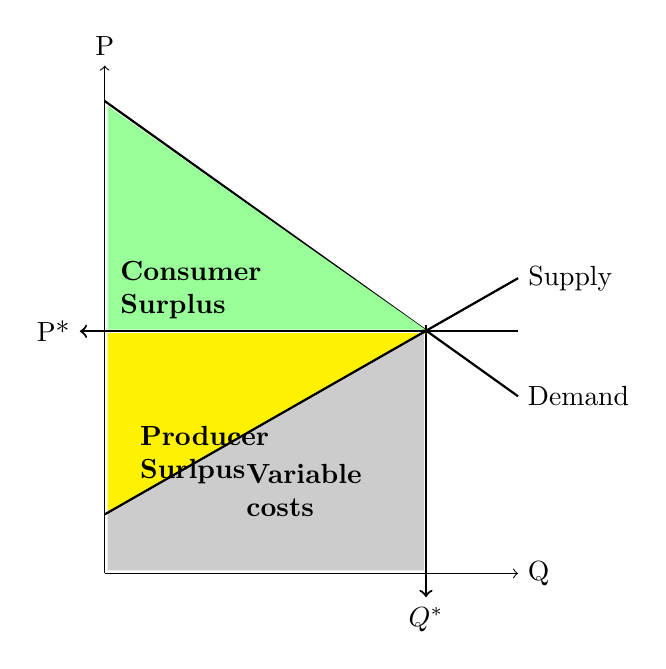
\begin{tikzpicture}[scale=1.5]
%\draw[thick,color=gray,step=.5cm, dashed] (-0.5,-.5) grid (3,3);
\draw[->] (0,0) -- (3.5,0) node[right ] {Q};
\draw[->] (0,0) -- (0,4.3) node [above] {P};
\draw[thick] (0,4) -- (3.5,1.5) ; \node [right]at (3.5, 1.5 ) {Demand}; 

\draw[thick,->] (2.72,2.1) -- (2.72,-.2) node[below] {$Q^*$};
\filldraw [color=green!40]  (0.03,2.07)-- (0.03,3.95)--(2.7,2.07)--cycle;
\filldraw [color=yellow] (0.03,2.03)-- (0.03,.515)--(2.7,2.03)--cycle;
\filldraw [color=gray!40](0.03,.515)--(2.7,2.03)-- (2.7,0.03)--(0.03,0.03)--cycle;
\draw[thick,<-] (-.21,2.05)node[left]{P*}  -- (3.5,2.05) node[above left] {}; 
%\fill[blue, opacity=.25]  (0,4) -- (1.86,2.1) --  (0,2.1) --cycle; 
%\fill[green] (0,.52) -- (1.82,2.1) --  (0,2.1) --cycle; 
\draw[thick] (0,.5) -- (3.5,2.5) node[right] {Supply};
\path (.7,2.4) node [text width=1.7cm](labelRent) {\textbf{Consumer\\ Surplus}};
\path (.8,1.) node [text width=1.5cm](labelRent) {\textbf{Producer\\ Surlpus}};
\path (1.7,.7) node [text width=1.5cm](labelvarcost){\textbf{Variable\\ costs}};
%\path (1.7,-1) node [black](labePC) {With producible capital};
  \end{tikzpicture}     
\caption{The basic supply and demand model determines price and quantity.}
\label{fig-equilibrium}
\end{center}
\end{figure}
LINK 2 STORIES---RENT HAS PERSISTED, BUT A BIG GAP -WE BRING IT BACK TO FILL THE GAP

\section{A new theory of urban rent for an age of human capacity}
suited to the economic reality---rising equality and wages following WWII. Massive inequality now..
we're in a new reality, but doesn't have a new economic theory for it. 

Late in the 20$^{th}$ century, the focus shifted again, to the economics of  knowledge, human capital, and how cities generate wealth, a change that plays a part in  our theory of urban rents in Chapter~\ref{chapter-growth}. 
 
The changes have tracked changing social relations. The influence of landowners declined and the power of  industrial capitalists increased throughout the 19$^{th}$ century. More recently the owners of industrial capital have been eclipsed, to some extent, by financial capital and by the owners or creators of certain information technologies.

We contribute to a modern theory centered on human capacity.

\subsection{Human capacity}
Change to neoclassical theory in economic tracked a change in the dominant mode of production, from primarily agricultural to primarily industrial.

We are now arguably in a third dominant mode of production, centered on  human capacity, (and computer/digital capacity). This is a new dominant mode of production but does not yet have a corresponding theory of distribution, and how that relates to production in space. 
This thesis works to fill that gap.\footnote{When a new dominant mode or age emerges, the old one doesn't go away. Stone work and bronze work still persist, agriculture and industrial production still persist, they are not however the force driving economic and social relations in the way the were when they were dominant as technologies and modes of production\cite{oldworldsdon'tdie}}

Rent is important in this new economy---and takes a rising share---Contradicting Marshall, Carey and Lachim \cite{careySomethingNothingHow2019} observe that,``[t]he persistent and growing profit share across a range of advanced economies and within industries fundamentally challenges the assumption of perfect competition and suggests that growing market power is at the heart of many of the economic challenges in America today.''


We address one set of problems by re-introducing rent in the classical sense within an urban model. 
We  use the neoclassical approach to distributing the distribution of the productive surplus to workers.

 % \Gls{class} structure, or how different classes participate in production changes over time as modes of production change. When Ricardo was writing, the economy was still largely reflected feudal social relations in that most land ownership originated in feudal military power. %Even the land of the nobility was divided up into smaller parcels run by knights or vassals. Both of these groups traded military support for land in the local manors. As higher ranking people, knights often presided over an entire manor, while vassals presided only over the land needed to support their families.
 % (IE DESCRIBE role of labour land, capital under feudalism and how this was changing in that period.) 
 
% ADD The evolution of the mode of production has continued, with human capital rather than land or industrial capital increasing the source of the social surplus. The concept of rent is specifically relate to surplus and enabled Ricardo to first talk about how is key to distribution within the economy, amongst classes.  Ricardo essentially developed his concept of Rent to explain the dynamics of distribution between classes. 
 
\section{Summary}


% MODE OF PRODUCTION
% STATE OF THE WORLD
% METHODOLOGICAL FRONTIER

% With the centrality  and the success of the neoclassical approach, with essentially a different underlying model of how the economy distributes surplus value, rent has played less of a central role.
We have examined the main stages of rent and distribution theory
% as  a bridge from classical rent theory to the
as the necessary background for our development %extension 
of a modern theory of urban rent. On the way we explained how the concept of economic rent arises in an agricultural economy, and who gets the rents in that type of economy. We then gave an account of how rent theory and the classical distribution theory was pushed into the background as neoclassical theorists analysed the industrial market economy that emerged after the industrial revolution, and introduced modern theories of production. In the next chapter we introduce 20$^{th}$ century urban models that are essentially an application of classical rent theory.

Neoclassical does..

% Clark's analysis of income distribution does 
The neoclassical approach does not contradict the classical view of rents, it simply displaces the analysis to the point where a competitive equilibrium prevails, and shifts attention away from the distribution of land rents. % Rents are not earned by the marginal unit of land and therefore the share to land at the margin is zero. 

What we do in our model is essentially these two stories of the distribution of the surplus, the rents, together in one model, in the urban economy, to take advantage of the strengths of both approaches, and make a model of %making and taking
urban production of value based on human capacity in cities with agglomeration effects. 
This brings the essentially spatial models of finance together with spatial models of urban rents, to model the effects of financialization. 

and makes it possible to talk formally in the neoclassical tradition with foundational questions of distribution, and with the older traditions of classical economics. 


% The distribution of rents in the urban model affects urban productivity in our model.
%***E FINANCIALIZATION IS ABOUT SURPLUS. CURRENT THINKING ABOUT FINANCIALIZATION HAS NOT BEEN NOT BEEN PUT INTO A FORMAL MODEL. FORMAL MODELS COME FROM COME FROM THE NEO-CLASSICAL TRADITION. 


